\documentclass[10pt,conference]{IEEEtran}

\usepackage{url,graphicx,subfigure,algcompatible,comment,amsmath,units,epsfig,threeparttable,multirow,colortbl,booktabs,setspace,textcomp}


\usepackage[ruled]{algorithm2e}

\title{Module Simulation-based Analog Placement Generation}
\author{
\IEEEauthorblockN{ Hung-Wen Huang\IEEEauthorrefmark{1}, Po-Cheng Pan\IEEEauthorrefmark{1}, Prof. Hung-Ming Chen\IEEEauthorrefmark{1}\\}
\IEEEauthorblockA{\IEEEauthorrefmark{1}Institute of Electronics and SoC Center, National Chiao Tung University, Hsinchu, Taiwan\\}
\IEEEauthorblockA{Email: nil113.cs00@nctu.edu.tw; benbean.ee96g@g2.nctu.edu.tw; hmchen@mail.nctu.edu.tw}

  %\thanks{
  %{\scriptsize
  %  This work was partially supported by the National Science Council of Taiwan ROC under grant No. NSC 102-2220-E-009-024
    

  %  \noindent
  %  978-1-4799-1071-7/13/\$31.00 \copyright2017 IEEE }
  %}
}

\begin{document}

\maketitle

\begin{abstract}

  The development of analog IC layout generation remains a challenge due to the imprecise estimation of circuit performance in advanced technology. However, the previous late-stage simulation results of modules can be reused for the purpose of mitigation of simulation gap in current analog placement generation. In this work, a new hierarchical flow is proposed to synthesize layout solutions based on the geometric preservation of user-defined constraints and previously generated layouts. The constraints of the circuit is priorly tackled in the partition and layout enumeration stage. In addition, we integrate the simulation and performance factors into the cost function in the layout enumeration strategy. The experiments show that this flow yields valid analog layout results whose performances are better than the those in previous approaches.

\end{abstract}

%\keywords{Partitioning, floorplanning, analog ICs, slicing tree, Physical Design, hMETIS, Defer, post-simulation}

\section{Introductions}\label{sec:intro}

Analog layout generation is commonly considered as difficult problem since the performance of analog circuit is sensitive to the process variations, and it is therefore strongly related to its geometric structure. In order to handle this problem, the designers present different constraints based on the circuit characteristics and design experiences. As the complexity of design grows in the advanced technology, manual layout design becomes impractical due to the lengthy design duration, which makes the research on automation of analog layout generation crucial. Recently, there are already several works about generating layout solutions fitting the constraints. However, applying constraints is merely an indirect attempt on the mitigation of the simulation gap. In other words, feasible performances in post-simulation are not always guaranteed. New methods other than geometric constraints should be considered in the modern approaches. 

\begin{figure}[ht]
    \begin{center}
    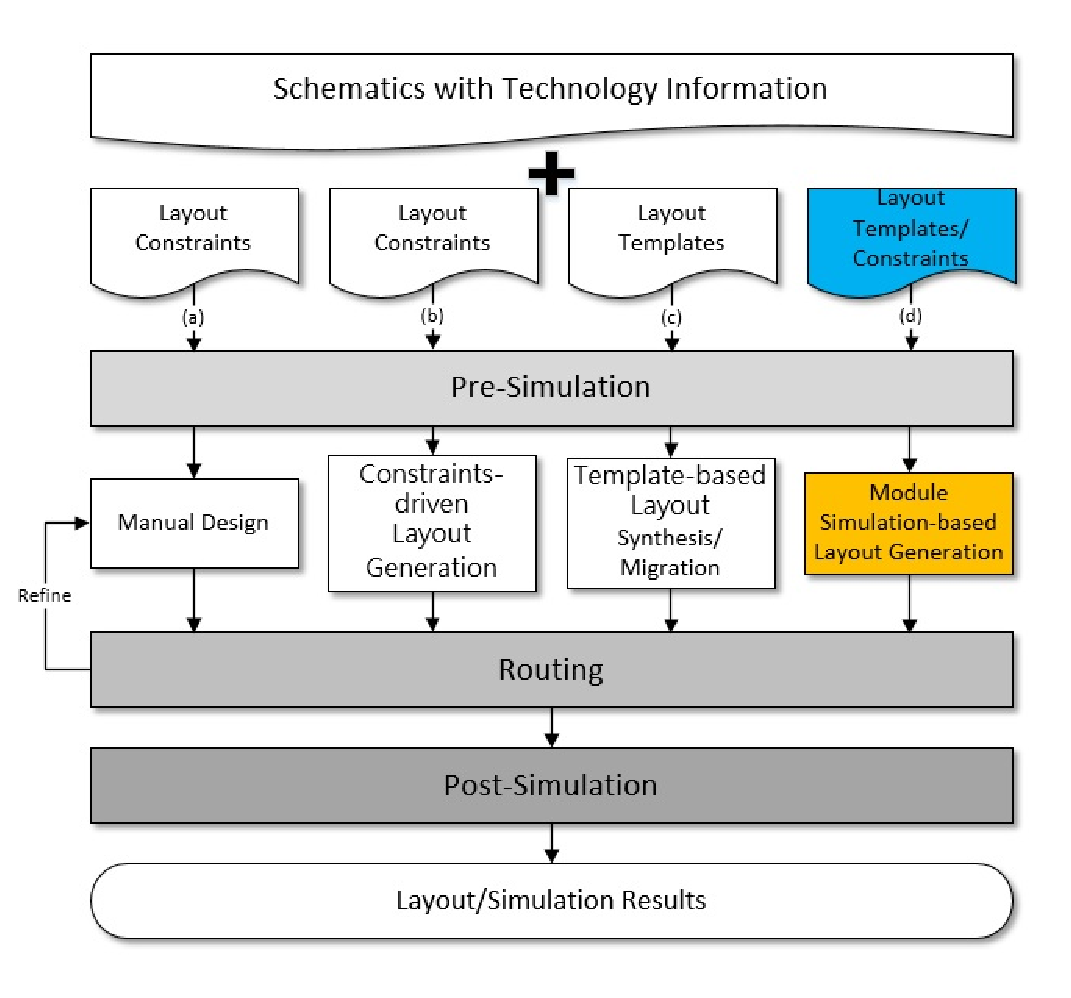
\includegraphics[width=0.5\textwidth]{Fig/Flow1.eps}
    \vspace{-1em}
    \caption{Illustration of layout generation with/without performance investigation} 
    \label{fig:Flow1}  
    \end{center}
    \vspace{-2em}
\end{figure}

In order to obtain the performances from the post-simulation, analog placement results are generated and then routed with manual effort. Originally, there are mainly three approaches to generate placement solutions from schematics. The first approach, as illustrated in Figure~\ref{fig:Flow1}(a), is the manual generation by the experienced designers. The designers iteratively refine the design until it turns feasible. Figure~\ref{fig:Flow1}(b) shows another approach, which is the layout-driven generation. The last approach shown in Figure~\ref{fig:Flow1}(c) is the migration based on the existing layout templates and modules. However, as mentioned in the upper, these approaches cannot directly reflect the 
precise simulation values in the layout solutions. Therefore, we proposed a new approach Figure~\ref{fig:Flow1}(d) which extracts both the previous layout templates and geometric constraints. Furthermore, it generates several module layout candidates and perform pairtial post-simulation. The simulation results are then fed back to the flow. In this way, the effect of simulation gap can be observed in much more earlier stage, and reduced by far. 

\subsection{Previous Works}

Existing approaches for analog layout generation are widely dicussed in the publication~\cite{Mark_ASPDAC16}. According to Figure~\ref{fig:Flow1}, the state-of-art analog layout generation methodologies can be roughly classified to two categories: (1) constraint-driven layout generation and (2) layout synthesis based on existing templates or previous layouts. Moreover, these approaches can be seperated into two classes according to their validation standard: (a) performance-oriented and (b) non-performance-oriented. The difference between two validation standard is whether their experimental results are from the complete post-simulation. In the following paragraph, the layout generation approaches are listed and classified in overview.

For the generation of the constraints-driven layout results, several data structures and algorithms of physical design are brought in and improved with perspective of physical characteristics of constraints. HB*-tree~\cite{Lin:2008uc}, Heterogeneous B*-tree~\cite{Chou:2011dj}, ASF-B*-trees\cite{PoHungLin:2009gx,Lin:2007vp}, extended ASF-B*-trees~\cite{Lin:2010vt}, TCCP~\cite{Lin:2011gz}, Simultaneous P\&R~\cite{SAPR_DAC13}, B*-tree considering linear constraints~\cite{Strasser:2008kf}, corner stitching compliant B*-tree~\cite{CBTree_ICCAD11} and QB-Tree~\cite{Wu:2016jw} handles various analog layout constraints, such as {\it symmetry, common centroid, proximity, regularity, thermal, current path and so on}. However, the performance in late-stage simulation is not well addressed in these approaches. On the other hand, ALG with Force-directed placement~\cite{AnaLayoutGen_TCAD09}, LAYGEN II~\cite{LAYGENII_TCAD13} and DeMixGen~\cite{Lin:2016dmg} generate layouts with constraints and address the experiment results with performances from post-simulation. As for the template-based layout synthesis or migration, migration approaches~\cite{Bhattacharya:cw,cart-hammouda-dac06,Jangkrajarng:2006cn,Zhang:2008fh,ZhengLiu:2010cy,Weng:2011gz,Chin_DMR_ICCAD2013,pcpan_adm_tcad15} and knowledge-based layout synthesis~\cite{Wu:2015ix,Lourenco:2016dv} are proposed in consideration of simulation performance, while~\cite{Wu:2015ds} is not. To sum up, there are already many works proposed to generate analog layout in both kind of approaches. None of the existing works takes advantage of both layout templates and constraints.


\subsection{Our Contributions}
\input{Preliminaries}
\input{Content}
\input{Experiments}
\input{Conclusion}

\bibliographystyle{IEEEtran}
\bibliography{IEEEfull,IEEEabrv,IEEEexample,Reference}

\end{document}